\chapter{Evaluating the impact of quality score calibration on variant calling}
\label{ch:evaluating}
\section{Introduction}

DNA sequencing is a powerful tool applied in many fields of biology. Understanding how DNA and changes in DNA influence organisms and how they interact with their environment is a fundamental goal of genetics. Correctly identifying the composition of a sampled DNA molecule is therefore an important first step for many genetic studies. However, this task is not trivial; sequencing technology is inherently prone to errors which can make it difficult to discern true biological effects from technical errors. 

Because of this error, the same piece of DNA is usually sequenced multiple times to attempt to get multiple measurements and a model is applied to infer the sample genotype. While a few sequencing errors do not impede accurate inference of the genotype of a monoploid sample, sequencing errors can be difficult to distinguish from heterozygosity in diploid organisms. This problem is even more difficult for samples with higher ploidy. However, using a statistical model enables a systematic approach to genotyping every site in the genome.

Additionally, a model allows the incorporation of auxiliary information when deciding the genotype at a site in a sample. For example, variant calling models often incorporate population genetic parameters that can help distinguish between sequencing errors and biological variation. The expected heterozygosity parameter \theta is particularly important; it usually paramaterizes some prior on the probability of a base matching the reference genome. If this deviates significantly from the true value, the model may mistakenly classify truly heterozygous sites as errors or vice versa.

The goal of using a model to call variants is to integrate a wide variety of information to make a principled decision about whether or not a variant exists. An important source of information on the trustworthiness of each sequenced base is the base quality score. This is a score, usually between 2 and 43, that encodes the probability the sequence is an error in the Phred scale. That is, the score $Q = -10\log_{10}P(\operatorname{Base is an error})$. This number is then rounded to the nearest integer and encoded as a character, shifted by 33, in the sequencing data.

Since these numbers can vary significantly in the same line with few patterns, quality scores can't usually be compressed very well by common compression algorithms. That gives sequencing data large filesizes that make it expensive to store the data for a lengthy period of time. Thus, these quality scores are often binned to reduce the amount of variation in the scores, enabling improved compression. Most binning methods attempt to do so in a way that minimizes the difference between the error rate of the bin and the error rate the bin should have according to its assigned score. However, there can still be a disconnect between the predicted error rate and the actual error rate. Furthermore, as the resolution of quality scores is reduced, some information about the true score at each base is lost.

To restore quality score resolution before analysis and to ensure quality scores accurately reflect the probability of error at every base, a process known as base quality score recalibration (BQSR) is sometimes performed. This attempts to use known information about sequencing errors to calibrate the quality scores. The most common method for doing so requires aligned reads and a set of variable sites that are removed from analysis. The algorithm then looks for bases that do not match the reference, assumes they are errors, and uses those errors to recalibrate the quality scores. See Chapter \ref{ch:kbbq} for more information on quality scores and base quality score recalibration.
	
The ultimate goal of quality scores and base quality score recalibration is to make it easier to identify erroneous bases, which should improve the set of variants a variant caller emits. However, evidence supporting the use of base quality score recalibration is limited and whether base quality score recalibration is worthwhile is subject to debate. The procedure has aided in detecting rare variants \parencite{ni_improvement_2016}, and a recalibration procedure that integrates mapping errors into quality scores seems to improve variant detection \parencite{li_improving_2011}. The goal of this chapter is to investigate the degree that base quality score recalibration affects variant calling to enable informed decisions for constructing variant calling pipelines, especially for non-model organisms.

\section{Methods}

I simulated datsets with various recalibration quality using GATK's BaseQualityRecalibrator \parencite{auwera_fastq_2013}, but with variable site sets that were artificially crafted to have different false positive and false negative calls, from 0 to 100 in steps of 20. The false positive rate of 100\% produced no output except in the case of 0\% false negative rate, which produced fewer calls than any other set. All datasets containing a 100\% false positive rate were therefore discarded.

This produced calibrations such that the higher the false negative and false positive rate, the less well-calibrated the output reads were. Refer to Chapter \ref{ch:kbbq} for more details on how the data was simulated and the CHM1-CHM13 truth set \parencite{li_synthetic-diploid_2018}. As a negative control, I compared each result to the raw, uncalibrated data. To see how the \texttt{kbbq} program affected variant calling, I also recalibrated the data with \texttt{kbbq}, with the options -\phantom{}-genomesize 214206308 and -a .15 .

I then called variants on each dataset using GATK HaplotypeCaller \parencite{poplin_scaling_2018} and evaluated the output SNP calls using RealTimeGenomics' RTG Tools vcfeval program \parencite{cleary_comparing_2015} and the truth set. I first ran the tool using the default settings, which also produces a ROC-like curve for the calls' GQ annotation. I also ran the tool using the -\phantom{}-vcf-score-field=QUAL option, which produces ROC-like curves for the site's QUAL annotation.

These curves are not strictly ROC curves since they plot the non-normalized number of false positives on the x-axis and the non-normalized number of true positives on the y-axis. In a true ROC plot, the false positive rate and true positive rate is plotted. However, they are similar and still show the shape of the trade-off between false positive rate and false negative rate. Since they are similar enough for the purposes of this analysis, I will refer to them as ROC plots.

This enabled comparison of the sensitivity and false positive rate trade-off of the two scores for each dataset. These two annotations were chosen because they represent an overall summary of the quality of the called variants.

%new paragraph
To evaluate the output calls, I plotted the number of false positive and true positive SNP calls for each dataset. I also constructed a heat map showing the F-measure of each dataset. This is the harmonic mean of the sensitivity and precision of the calls and is one way to summarize the accuracy of the calls.

%new paragraph
%Filter info + justifications:
%#filter: only snps
%#filter: DP > 35 & DP < 65 (+-2 SDEV from mean of ~50 assuming poisson)
%#filter: QUAL > 75; this is ~bottom 1% and the maximum F
%#   value from the previous analysis is between 75 and 150.
To see how filtering the calls affected their quality, I then identically filtered each variant set with two filters using bcftools view \parencite{li_sequence_2009}. The first filter is a depth filter, only accepting variants that have more than 35 aligned reads and fewer than 65. This is within two standard deviations of the mean sequencing depth of \~50, assuming the read depths are Poisson distributed. The second filter is a QUAL filter, accepting only calls with a QUAL of over 75. This threshold was chosen because it is approximately the bottom 1\% of QUAL values in each dataset and it is the lowest QUAL value that maximizes the F-measure of all the datasets. I then calculated the same statistics and made the same plots using the filtered calls.

%THE STORY IS COMING TOGETHER: The range in number of TP calls grows after filtering! Prior to filtering there is a big difference in the number of FPs in each dataset (1009), but this difference shrinks after filtering to 548. The difference in number of true positives starts at 240, but grows to 2044 after filtering.
%TODO: fix figure sizes and title line breaks.
%TODO: add precision/recall numbers
%TODO: add TP/FP and prec/recall range differences to text
%TODO: add in the raw, uncalibrated data and see where that falls.

% /storage/2017-03-15-eucalyptus/2020-09-28-kbbqflt
Finally, I ran the kbbq software (see Chapter \ref{ch:kbbq}) with the specified genome size 605951511 and coverage 240 to recalibrate a set of reads sequenced from an individual of the non-model species \textit{Eucalyptus melliodora} \parencite{orr_phylogenomic_2020}. This dataset contains reads from 3 leaves each from 8 branches, each leaf sequenced to a depth of approximately 10X. I then called variants using HaplotypeCaller and filtered the calls using the same filters from \cite{orr_phylogenomic_2020}. At each filtering step, I took the approach described in Chapter \ref{ch:structured} to estimate the false discovery rate and false negative rate. Briefly, I created 100 random trees that were maximally distant from the true tree structure and filtered using these random trees instead of the true tree. Any variants that appeared in any of the randomized trees but not in the set of variants identified in \cite{orr_phylogenomic_2020}, I classified as false positives. To estimate the false negative rate, I counted the number of variants in the previously identified calls that were not found via the reference-free caller. I then compared these values to those found in \cite{orr_phylogenomic_2020}.

\section{Results}

To evaluate the output calls, I plotted the number of true positives and false positives for each dataset recalibrated using sets of variable sites with differing false negative and false negative rates (Figure \ref{fig:vc_fptp}). This shows that improved calibration increases the number of true positive variants called. However, improved calibration also increases the number of false positives. More detail about the relationship between false positives and negatives in the database of calibrated sites are shown in the heat maps in Figure \ref{fig:vc_p}.


\begin{figure}
\centering
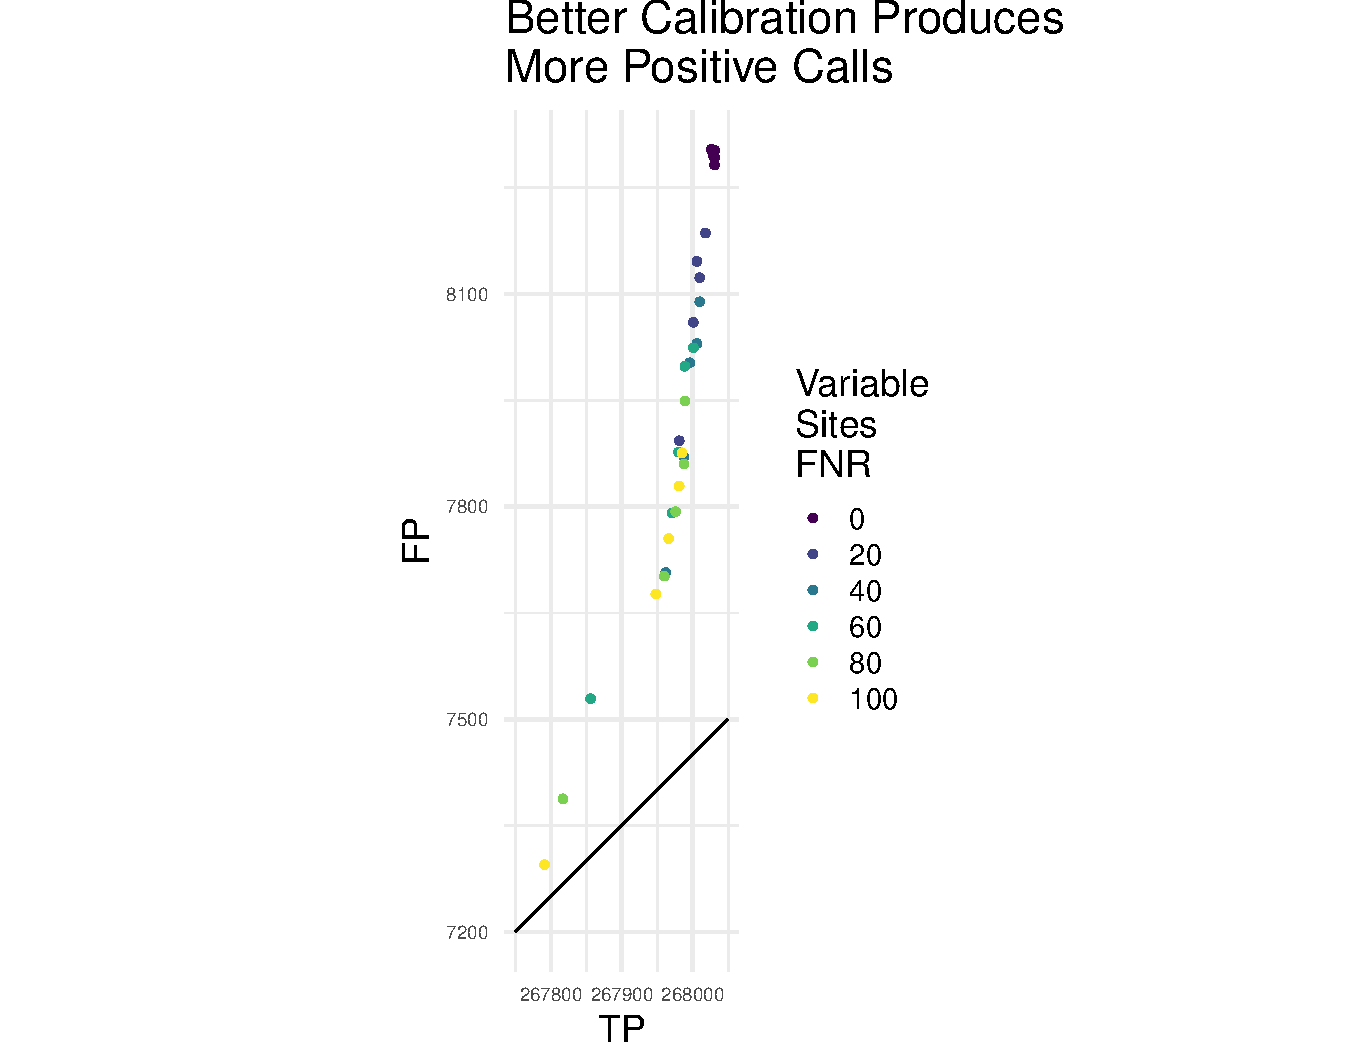
\includegraphics[width = .8\textwidth]{tp_fp_plot.pdf}
\titlecaption{Unfiltered True Positive and False Positive Calls}{The output number of positive calls for each dataset. The false negative rate of the set of variable sites used to calibrate the reads used to produce each callset is shown. As the false negative rate decreases, the number of both true positive and false positive calls increases.}
\label{fig:vc_fptp}
\end{figure}

\begin{figure}
\centering
\includetwo{fp_heatmap.pdf}{tp_heatmap.pdf}
\titlecaption{Unfiltered Positives Heatmap}{The output number of false positive calls for each dataset. The false negative and false positive rate of the set of variable sites used to calibrate the input reads is shown on the x and y axis. The color of each cell represents the number of unfiltered false positive (left) or true positive (right) SNP calls. As the false negative and positive rates decrease, the base quality scores become more calibrated, and more calibrated data produces more false positive and true positive calls.}
\label{fig:vc_p}
\end{figure}

To determine the impact of these variants on the overall quality of the callsets, I constructed heatmaps of the sensitivity and precision of each dataset (Figure \ref{fig:vc_sens_prech}). As the data become more well-calibrated, the sensitivity of the caller increases; however, the precision of the caller also increases. This means that the caller is able to detect more true variants, but a higher proportion of the calls it makes are false positives. To visualize the trade-off between sensitivity and precision, I plotted the precision against the sensitivity of each dataset, shown in Figure \ref{fig:vc_sens_prec}. To summarize the overall effect on accuracy, I show how the F-measure changes across each dataset in Figure \ref{fig:vc_f_heatmap}.

\begin{figure}
\centering
\includetwo{sensitivity.pdf}{precision.pdf}
\titlecaption{Unfiltered Sensitivity and Precision Heatmaps}{The sensitivity (left) and precision (right) of the variant caller on each dataset with no filtering. As the base quality score calibration of the input reads increases, the sensitivity of the caller increases and the precision decreases.}
\label{fig:vc_sens_prech}
\end{figure}

\begin{figure}
\centering
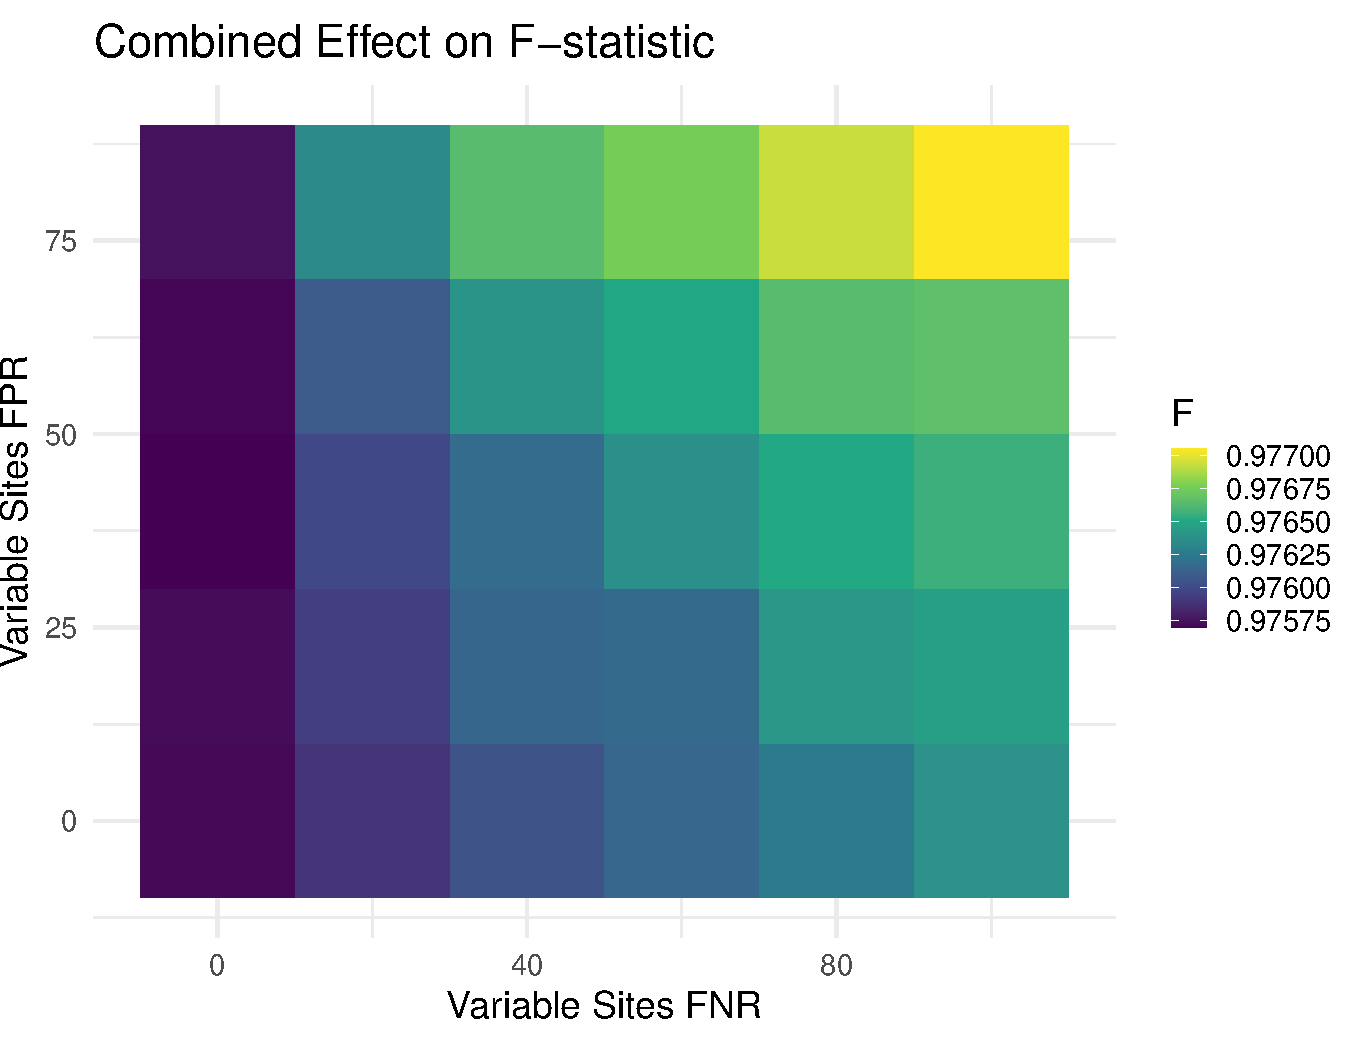
\includegraphics[width = .8\textwidth]{f_heatmap.pdf}
\titlecaption{F-measure of Unfiltered Calls}{The F-measure of the unfiltered calls of each dataset. As the base quality score calibration of the input reads increases, the F-measure of the caller decreases. This is driven by the fact that the increase in sensitivity of the caller is much smaller than the decrease in precision.}
\label{fig:vc_f_heatmap}
\end{figure}

Since the base quality score of the reads used to support each genotype call evidently play a role in whether to emit a variant, I wanted to see how the differences in calibration affected the annotations output by the caller. To that end, I plotted a ROC-like curve showing how the number of false positive and false negative calls for variants filtered according to the QUAL and GQ (Figure \ref{fig:vc_rocs}) annotations. These are both statistics that summarize the quality of the emitted site in a single, increasing score, and so are well-suited for ROC analysis. According to the VCF standard, the QUAL score is a phred-scaled probability that the ALT allele(s) present in the call are not actually present, $P($ALT is wrong$)$. The GQ score is the phred-scaled conditional probability the genotype call is incorrect given the site is variable, $P($genotype is wrong $|$ site is variant$)$.

\begin{figure}
\centering
\includetwo{qualroc.pdf}{gqroc.pdf}
\titlecaption{Unfiltered ROC Curves}{The ROC curves for the QUAL (left) and GQ (right) score of an output call for the unfiltered calls of each dataset. The color of each line represents the false negative rate of the set of variant sites used as input to recalibrate the reads used to call variants. Each point in the line represents the number of false positive and false negative calls that have a score above the QUAL or GQ threshold for that point. As this threshold decreases, the number of false positives and true positives increases, though at different rates. These plots show that as the false positive rate increases, the number of true positive calls increases at a faster rate for the well-calibrated data than in other datasets for the QUAL classifier, but at a slower rate for the GQ classifier.}
\label{fig:vc_rocs}
\end{figure}

As the ROC plots show that each dataset would respond to filtering differently, I examined how the calls would improve or not after filtration. Since the ROC curves show each dataset would respond differently to a QUAL filter, I used a small QUAL filter filtering out variants with the lower 1\% of QUAL scores. This percentage coincides with the smallest QUAL value of the QUAL values that maximize the F-measure of every dataset. These values are shown in Figure \ref{fig:vc_f_heatmap}. Depth filters are very common after variant calling, so I also used a depth filter to filter out calls that had unusually high or low depth.

This resulted in a similar pattern of positive calls as the unfiltered data, seen in Figure \ref{fig:vc_flt_p}; better calibrated data had more false positive and true positive calls. However, the difference between the number of true positive variants called from best-calibrated data and worst-calibrated was much larger after filtration. Before filtering, the largest difference between datasets was 240 true positive calls; this difference grows to 2044 after filtering. The opposite is observed for the false positive calls: before filtering, the largest difference in the number of false positive calls was 1009, but after filtering this difference decreases to 548. 
% Additionally, the difference between the number of true positives in the best-calibrated data and the next-best calibration at each step was smaller. So filtering caused even imperfectly-calibrated data to behave more like well-calibrated data, even though the extremes were further apart.                  %<- this is kinda weak
Ultimately, this alters the sensitivity and precision of each dataset such that the range of the sensitivity is increased and the range of the precision is decreased (see Figure \ref{fig:vc_flt_p}). This is sufficient to make the best-calibrated data also have the best F-measure of all the datasets, shown in Figure \ref{fig:vc_flt_f}.

\begin{figure}
\centering
\includetwo{flt_fp_heatmap.pdf}{flt_tp_heatmap.pdf}
\titlecaption{Filtered Positive Calls}{The output number of false positive and true positive calls for each dataset. The false negative and false positive rate of the set of variable sites used to calibrate the input reads is shown on the x and y axis. The color of each cell represents the number of false or true positive SNPs after filtering. As base quality scores become more calibrated, the number of positive calls increases. Note the range of positive calls has increased in comparison to each unfiltered dataset. Before filtering, the difference in the number of true positives between datasets was at most 240; after filtering it rises to 2044.}
\label{fig:vc_flt_p}
\end{figure}

% > rangedif(df$precision)
% [1] 0.003542063
% > rangedif(fltdf$precision)
% [1] 0.002312442
% > rangedif(df$recall)
% [1] 0.0008826549
% > rangedif(fltdf$recall)
% [1] 0.00748611

\begin{figure}
\centering
\includetwo{flt_sensitivity.pdf}{flt_precision.pdf}
\titlecaption{Filtered Call Sensitivity and Precision}{The sensitivity (left) and precision (right) of the variant caller on each dataset after filtering. As the base quality score calibration increases, the sensitivity of the caller increases and the precision decreases, as seen in the unfiltered data. However, the difference between the largest and smallest precision is slightly smaller than in the unfiltered data, and the difference between the largest and smallest recall is much larger.}
\label{fig:vc_flt_sp}
\end{figure}

\begin{figure}
\centering
\includetwo{sens_precision.pdf}{flt_sens_precision.pdf}
\titlecaption{Sensitivity and Precision Before and After Filtering}{The sensitivity and precision of the variant caller on each dataset with no filtering on the left, and after filters are applied on the right. In the unfiltered calls, as the base quality score calibration of the input reads decrease, the sensitivity of the caller decreases but its precision increases. Once the calls are filtered, the same pattern is observed. However, after filtering the range of precision between datasets is much smaller than before filtering. Conversely, the range of sensitivity increases.}
\label{fig:vc_sens_prec}
\end{figure}

\begin{figure}
\centering
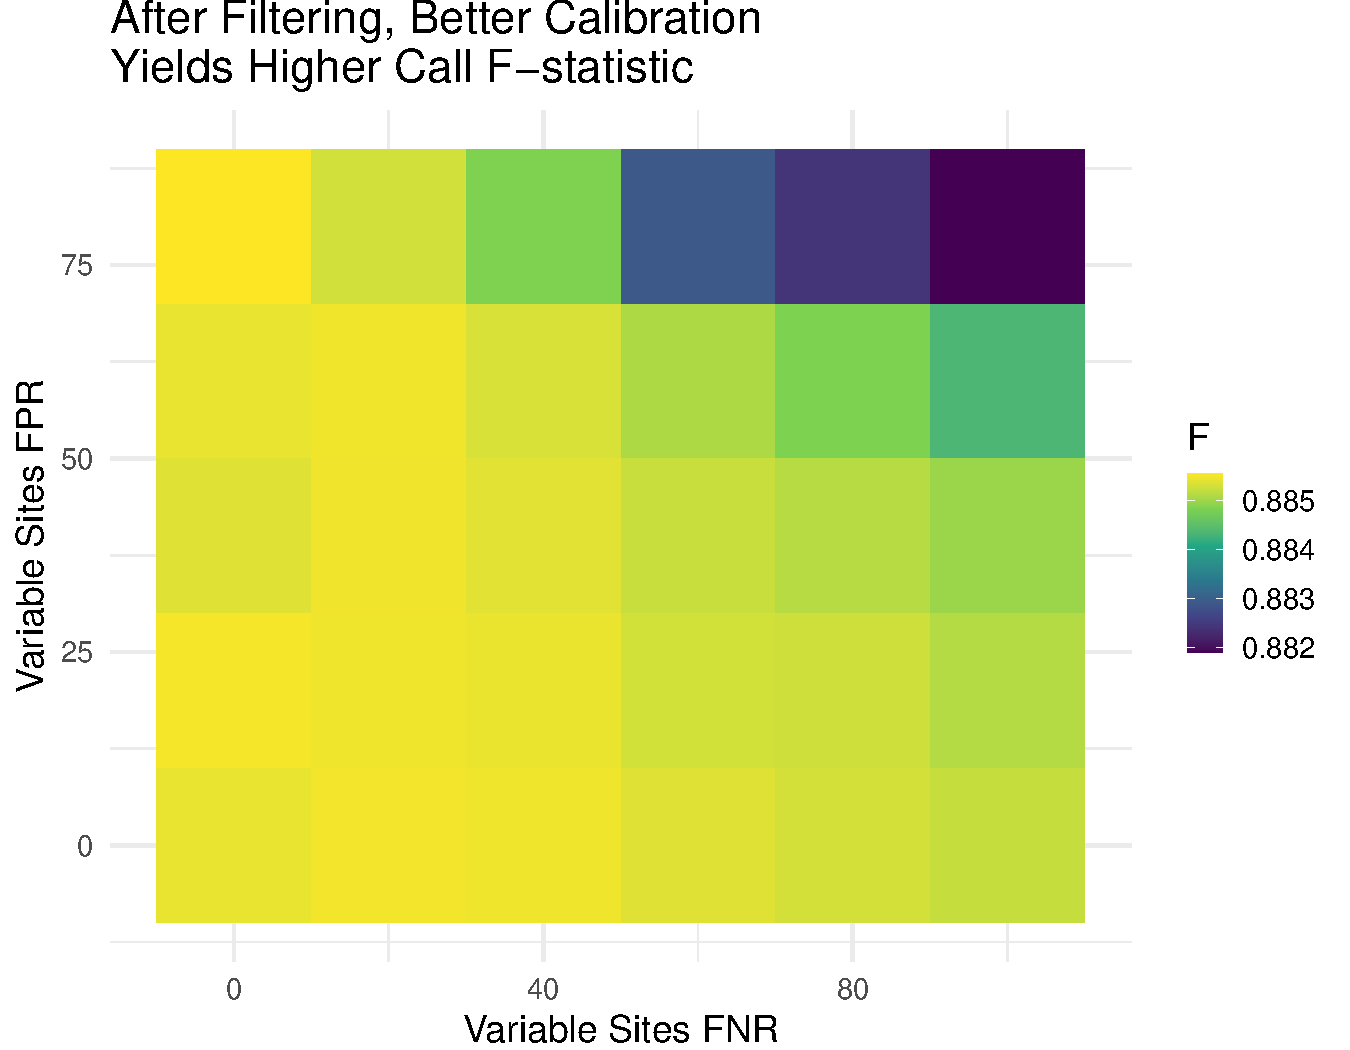
\includegraphics[width=.7\linewidth]{flt_f_heatmap.pdf}
\titlecaption{Filtered F-measure}{The F-measure of each dataset. As the calibration of the data improves, so does the F-measure. This is in contrast to the unfiltered data, in which the worst-calibrated data has the best F-measure. This difference is driven by an increase in relative precision of the best-calibrated data and a decrease in relative sensitivity of the poorly-calibrated data.}
\label{fig:vc_flt_f}
\end{figure}

%TODO: fix figure sizes and title line breaks. combine similar plots into 1 figure to make the whole chapter more readable
%TODO: add in the raw, uncalibrated data and see where that falls.

\subsection{Variants Detected With KBBQ Recalibrated Reads}

In order to determine the effect of reference-free recalibration on variant calls, I recalibrated the reads with the reference-free base quality score recalibrator KBBQ (see Chapter \ref{ch:kbbq} for more information on KBBQ). I then called variants and filtered the same way they were called and filtered in \cite{orr_phylogenomic_2020}. The number of variants called at each step in the filtering process is shown in Table \ref{tbl:num_variants}. After filtering, 106 variants were detected; 34 of these were also detected in the confident set of variants previously identified. This previous set had a total of 90 variants. Filtering reduced the average number of false positive variants estimated to 35.54. Note that the number of detected sites listed in Table \ref{tbl:num_variants} are not all indicative of mutation, as the number includes heterozygous sites until the last filtering step.

\begin{table}
\begin{tabularx}{\textwidth}{>{\hsize=1.5\hsize\linewidth=\hsize}X >{\hsize=.7\hsize\linewidth=\hsize}X >{\hsize=.9\hsize\linewidth=\hsize}X >{\hsize=.9\hsize\linewidth=\hsize}X}
\toprule
\textbf{Description} & \textbf{Num} & \textbf{Estimated} & \textbf{True}\\
& \textbf{Variants} & \textbf{False Positives} & \textbf{Positives} \\
\midrule
Appears in first 11 scaffolds & 9838408 & 911.46 & 88\\
Total depth <= 500 & 9190223 & 800.83 & 87\\
ExcessHet <= 40 & 4932628 & 144.95 & 86\\
Not within 50bp of an indel & 3175128 & 85.05 & 69\\
Biallelic SNPs & 1913594 & 68.88 & 67\\
Outside repeat regions & 857810 & 35.54 & 46\\
All 3 replicates match & 63793 & - & 35\\
Only variable sites & 106 & - & 34\\
\bottomrule
\end{tabularx}
\titlecaption{Number of Detected Variants After KBBQ Recalibration}{The number of variants detected at each step in the filtering pipeline. Each row includes a description of each filter and the number of variants remaining after the filter has been applied. It also includes the number of false positives estimated by simulating 100 random, maximally distant trees, using those trees to filter the result at each step, and averaging the number of variants that survive filtering. Since step 7 includes filtering based on replicate agreement, this method cannot detect false positives for step 7 or 8; in the worst case, they are identical to the number of estimated false positives in step 6. True positives were estimated using the number of variants ultimately detected in the confident set described in \cite{orr_phylogenomic_2020}. This set contains a total of 90 variants.}
\label{tbl:num_variants}
\end{table}

\section{Discussion}

%todo: talk about F statistics
%todo: discuss e mel results

Overall, these results show that as the quality of the calibration increases, the quality of the variant calls also slightly increases. The difference is very small, but better calibration produces more positive calls, with more true positive calls than any other dataset. And though I only filtered the data with two fairly lenient filters, the best calibrations still produced the most true positive calls of any dataset.

Interestingly, filtering seemed to amplify the difference between well-calibrated and poorly-calibrated data, increasing the disparity in the number of true positive variants detected. At the same time, filtering reduced the disparity in the number of false positive variants identified.

%Talk about how filtering becomes very important for leveraging the power of calibration
This observation makes filtering very important for variant calling. Variant callers will generally prefer to include a putative variant rather than exclude it and miss a truly variant site. Thus, they prefer sensitivity over precision. The reason for this preference can be seen in Figure \ref{fig:vc_sens_prec}, where filtering reduced the sensitivity of every set of calls but greatly improved precision and decreased the range of precision values. Filtering raw calls is paramount to getting a variant set with acceptable levels of sensitivity and precision. Ultimately, the impact of base quality score recalibration is not going to be as large as the filters one chooses to use. In this case, better calibration results in an increased precision of \~.003 before filtering; filtering itself increased precision by about .08, while reducing sensitivity by approximately .18. So the effect of calibration on sensitivity and precision is small in comparison. At the same time, if the variant that matters for the purposes of the study being conducted, this difference in calibration could be important.

Unfortunately, this means that filtering plays a big role in the success of a variant calling pipeline. While there is no definitive best way to filter variants in all cases, Figure \ref{fig:vc_rocs} shows that differences in quality score calibration can affect the annotations attached to each call and make the same filters more or less effective, depending on the threshold used. While this is interesting, it doesn't necessarily change how filtering should be done or suggest an optimal filtering strategy.

One limitation of this study is that is uses only a single dataset and only a sparce range of false positives and false negatives in the database of variable sites. Especially since the effect of calibration on the output variant calls is small, a different dataset may yield different results. As seen in Chapter \ref{ch:kbbq}, the calibration of the raw reads in this dataset is not particularly bad. Furthermore, this data is from a human-derived cell line, and protocols for DNA extraction and sequencing are fairly well-established. Additionally, the original base calling algorithm is likely tuned to work well with human-like data. All together, this means that while the effect of recalibration was not particularly pronounced in this dataset, base quality score recalibration may have a higher impact on data that is messier, contains more errors induced in sample preparation, or results from failed sequencing runs. Replication with other datasets and other variant callers is necessary to further elucidate the role of base quality score calibration on variant caller performance.  
%Talk about how BQSR actually made everything worse!!!

%Speculate about when BQSR might actually be useful!! More work is needeD!!!

% Surprisingly, the behavior of the raw dataset is most similar to that of KBBQ and the dataset calibrated with perfect information. At the same time, the patterns observed clearly indicate an effect of calibration on how HaplotypeCaller functions. This can be explained in a few ways; 1) GATK's own calibration method is flawed, and the raw data is truly the best calibrated data, so the trends are real. 2) this dataset is just weird 3) the calibration is actually correct and calibration affects HC in a roundabout way that doesn't directly translate into better calls. The trends are an artifact of that process.

\subsection{KBBQ Recalibration Improved \textit{E. melliodora} Calls}

While the simulated datasets revealed a complex interaction between the number of detected variants, sensitivity, precision, and filtering, it appears KBBQ recalibration improved the ability to successfully call variants in a non-model organism. In Chapter \ref{ch:kbbq}, I showed that using GATK's recommended approach of calling confident variants and using those as the set of variable sites to use in recalibration results in poor base quality score calibration. I also showed that using the KBBQ method improved calibration to near-perfect GATK recalibrations. The calls on the simulated datasets shown here also imply that KBBQ recalibrated reads behave similarly to or better than reads recalibrated with GATK using perfect information.

Using the same calling and filtering parameters as those used in \cite{orr_phylogenomic_2020} yielded more variants at the end of filtering with 106 instead of 99. This is consistent with the results from the simulated datasets, where better-calibrated data yields more variant calls. Indeed, this is the case even before other filters are applied, with 9,838,408 variants detected versus 9,679,544 detected in the prior study. Additionally, the number of variants after filtering that appear in the confident set identified in the previous study increased from 30 to 34. However, in contrast to the results from the simulated data, the number of estimated false positive calls decreased as well in the KBBQ recalibrated data, falling from 55.71 to 35.54 after filtering and from 1033.18 to 911.46 before filtering. Thus, using KBBQ to recalibrate the reads before calling seems to have increased both the sensitivity and the precision of the variant calling pipeline.

After all filters were applied, the pipeline yielded 106 mutations with an estimated 36 false positives and 34 previously-estimated true positives. This leaves approximately 36 positive variants that were not in the set of previously identified variants. This is an approximately 2.8 times increase from that same estimate of 13 inferred with the calls from \ref{orr_phylogenomic_2020}. While this is an estimate based on the false positive rate and so cannot be used to distinguish between previously unidentified true variants and false positives, it shows how the decrease in false positive rate from using KBBQ recalibrated reads improves the overall ability of the variant calling pipeline to reveal true mutations.

% Why might the empirical results differ from the simulated ones?

% TODO: run the pipeline on the raw reads and see what the difference is (ie not use GATK calibration)

\section{Conclusion}

The simulated data here shows that quality scores do have a small but important effect on the quality of the called variants. This manifests itself in not only the difference in the number of true positive calls and the number of false positive calls, but also in the QUAL and GQ annotations. At the same time, the size of the effect is small. While effective recalibration will certainly benefit variant calling, even somewhat large errors in the input variable sites will not significantly hurt the performance of HaplotypeCaller. If very high sensitivity is critical to the analysis being performed, care must be taken to ensure that base quality scores are properly calibrated.

\printbibliography
